\documentclass[conference]{IEEEtran}
\IEEEoverridecommandlockouts
% The preceding line is only needed to identify funding in the first footnote. If that is unneeded, please comment it out.
\usepackage{cite}
\usepackage{amsmath,amssymb,amsfonts}
\usepackage{graphicx}
\usepackage{textcomp}
\usepackage{xcolor}
\usepackage{algorithmic, algorithm}
\def\BibTeX{{\rm B\kern-.05em{\sc i\kern-.025em b}\kern-.08em
    T\kern-.1667em\lower.7ex\hbox{E}\kern-.125emX}}
\begin{document}

\title{ Sequential algorithm to split, merge and resplit multidimensional arrays }

\author{\IEEEauthorblockN{1\textsuperscript{st} Timothée Guédon}
\IEEEauthorblockA{\textit{Department of Computer Science and Software Engineering} \\
\textit{Concordia University}\\
Montreal, Quebec, Canada \\
t\_guedon@encs.concordia.ca}
\and
\IEEEauthorblockN{2\textsuperscript{nd} Tristan Glatard}
\IEEEauthorblockA{\textit{Department of Computer Science and Software Engineering} \\
\textit{Concordia University}\\
Montreal, Quebec, Canada \\
tristan.glatard@concordia.ca}
\and
\IEEEauthorblockN{3\textsuperscript{rd} Valérie Hayot-Sasson}
\IEEEauthorblockA{\textit{Department of Computer Science and Software Engineering} \\
\textit{Concordia University}\\
Montreal, Quebec, Canada \\
email address or ORCID}
}

\maketitle

\begin{abstract}
This document is a model and instructions for \LaTeX.
This and the IEEEtran.cls file define the components of your paper [title, text, heads, etc.]. *CRITICAL: Do Not Use Symbols, Special Characters, Footnotes,
or Math in Paper Title or Abstract.
\end{abstract}

\begin{IEEEkeywords}
component, formatting, style, styling, insert
\end{IEEEkeywords}

%----------------------------------------
\section*{Introduction}
%----------------------------------------

\subsection{Context}

With the improvement of aquisition methods in several scientific domains like health sciences, geology and astrophysics, processing a deluge of very high resolution images has become a Big Data challenge. Most pipelines process only specific ROI or process data by block. At the end of the pipeline, merging those blocks into one file may be required as well. Previous work in \cite{seqalgorithms} introduced two types of sequential algorithms to split and merge very high resolution images: the ``clustered" and ``multiple" strategies. In this paper, we define a new algorithm to resplit data that has already been splitted before into an other shape, and we show that it can also be used to split and merge data with the same behavior of the ``multiple" strategy. We also give an implementation of this algorithm, available as an optimization package for the Python big data library ``Dask".

\subsection{Problem definition}

Consider a multidimensional array of shape $R = (R_i, R_j, R_k)$, stored in some input files with a given shape $I = (I_i, I_j, I_k)$, all input files having the same shape.
Our goal is to optimize the process of sequentially resplitting the input files into output files with a different shape $O = (O_i, O_j, O_k)$, all output files having the same shape, too. \\

The resplit process has two particular cases:
\begin{itemize}
  \item It becomes a split process if there is one input file and several output files,
  \item It becomes a merge process if there are several input files and one output file.
\end{itemize}

For this I/O process to be fast, one needs to minimize the number of seeks that occur on disk while reading and writing.
We consider that a seek occurs either when opening a file or seeking into a file. \\

Let us consider a basic sequential resplit algorithm: One can repeatedly read the maximum amount of data possible from the input files into a buffer stored in main memory, and then write this buffer down into the output files requiring this data, until all output files have been completely written.
This resplit algorithm is described in Algorithm \ref{algo:generalresplit}. \\

Given Algorithm \ref{algo:generalresplit}, the optimization problem that we want to solve can be stated as follows:
Given the amount of main memory available $m$, as well as the shapes of the input and output files $I$ and $O$, how to select the best buffer shape $B$ which will minimize the number of seeks that take place during reading and writing? \\

We add two restrictions on the buffers: We shall use only non-overlaping buffers, all buffers having the same size, and each buffer has to be written only once.

\begin{algorithm}[H]
  \caption{Basic resplit algorithm}
  \label{algo:generalresplit}
  \begin{algorithmic}
    \STATE \textbf{Inputs:} {inFiles, outFiles, m, buffersList}
    \FOR{$\textrm{buffer in buffersList}$}
      \STATE $\textrm{read(inFiles, buffer)}$
      \STATE $\textrm{write(outFiles, buffer)}$
    \ENDFOR

  \end{algorithmic}
\end{algorithm}

\subsubsection{Consistency with previous works}
For the sake of consistency with previous works \cite{seqalgorithms}, we call the original array of shape $R$ stored in the input files the ``reconstructed image" (see Figure \ref{fig:reconstructed_img_divided}).
Of course, the input files' positions in the reconstructed image have to be stored in some way.
Also with a view to be consistent with previous works, we assume the files to be written in column-order.
In column ordering (also called ``F" ordering) the fastest moving dimension is the last dimension of the array and the slowest moving dimension is the first dimension.
For example a 3D array with dimensions i, j and k would be written on disk by writing the complete columns in the k dimension first (see Figure \ref{fig:column_order}).

\begin{figure}[h!]
\centering
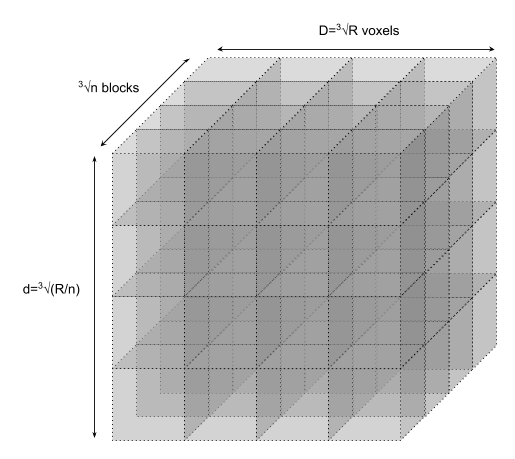
\includegraphics[scale=0.3]{./figures/reconstructed_img_divided.png}
\caption{Illustration of the reconstructed image divided into input files at the initialization of the resplit algorithm.
}
\label{fig:reconstructed_img_divided}
\end{figure}

\begin{figure*}[h!]
\centering
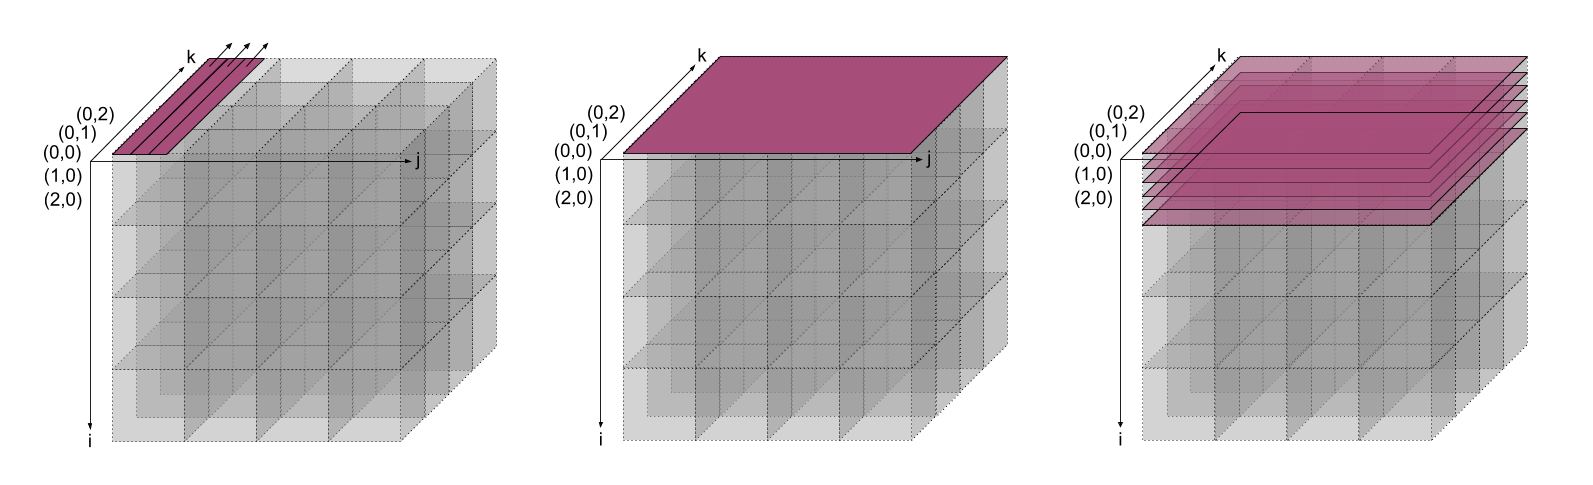
\includegraphics[scale=0.25]{./figures/column_order.png}
\caption{Illustration of the column-order storage of voxels in a file.
}
\label{fig:column_order}
\end{figure*}

\subsubsection{Details of the sequential resplit algorithm}
The algorithm described in Algorithm \ref{algo:generalresplit} takes a list of input and output files $inFiles$ and $outFiles$ as parameters, as well as the amount of memory $m$ available in RAM for the buffer and the list of the buffers' coordinates. We call $m'$ the amount of memory available in the buffer at a given time during the execution of the algorithm ($m'=m$ at initialization). The list of buffers' coordinates contains the coordinates of each buffer to be loaded in the referential of the reconstructed image. \\

The algorithm successively loads as much data as it can from the input files into the buffer and write it down to the output files that are supposed to contain this data.
Although we could use a naive shape for the buffer, we can use the input and output files shapes to elaborate more efficient strategies as we will see in the next sections.
The algorithm ends when all buffers have been read.
Therefore, the buffers must cover the whole reconstructed image such that when the algorithm end all the output files have been completely written.
For the latter statement to be true, we also need to ensure that all data read from input files are either stored in RAM or directly written, such that all the output files are completely written at the end of the algorithm.

\subsection{Naive algorithm}

As a base case for our problem, let us define a naive algorithm which loads one input file at a time and write it down into the different output files that requires the data.
The buffers have the same shape as the input files ($B=I$) and the order is the same order than the storage order i.e. the column order in this study ($[k, j, i]$ order).
% TODO : seeks analysis

\subsection{A particular case}

If the input shape is a multiple of the output shape such that one input file covers several output files entirely without falls, then the problem is easily solved: one must read as much input files as one, i.e. the buffer shape $B$ is a multiple of the input shape $I$.
The algorithm will produce one seek per input file and one seek to write each output file, which is the minimum number of seeks possible for a resplit.\\

If there is a mismatch between the shapes in any dimension however, one needs a strategy to manage with this overlap while minimizing the number of seeks.
We will introduce a strategy to keep falls temporarily into memory in the next section, this strategy's efficiency is completely dependent on the amount of main memory available. \\

Also, the resplit process requires multiple buffers to be read.
If there is no overlap between input and output files, then the order in which we load buffers is not important.
In case of an overlap however, the order may have an important impact on the number of seeks produced.

%----------------------------------------
\section*{Notations}
%----------------------------------------

\begin{tabular}{ c | l }
  $m$    & Amount of main memory available for the buffer at initialization \\
  $m'$    & Amount of main memory available for the buffer during the algorithm execution \\
  $\textrm{iterable}[i]$ & Access the $i^{th}$ element of an iterable \\
  $B = (B_i, B_j, B_k)$ & Shape of the buffer \\
  $(B_i B_j B_k)$ & Size of the buffer in voxels \\
  $R_i, R_j, R_k$   & Length of the reconstructed image in the $i^{th}$ dimension \\
  $I_i, I_j, I_k$   & Length of an input file in the $i^{th}$ dimension \\
  $O_i, O_j, O_k$   & Length of an output file in the $i^{th}$ dimension \\
  $C_i(x), C_j(x), C_k(x)$    & Overlap size in voxels in the $i^{th}$ dimension, when loading the $t^{th}$ buffer. \\
  $\Lambda_i, \Lambda_j, \Lambda_k$    & Length of an input aggregate in the $i^{th}$ dimension \\
  $\Omega_i, \Omega_j, \Omega_k$    & Length of an output aggregate in the $i^{th}$ dimension \\
  $b_i, b_j, b_k = \frac{R_i}{B_i}$    & The number of buffers in the $i^{th}$ dimension in the reconstructed image \\
  $f_1, f_2, f_3$   & Names of the overlap areas in 2D \\
  $F_1, F_2, F_3, F_4$   & Names of the overlap volumes in 3D \\
  $ N_s $    & Number of buffers in a slice \\
  $ n_s $    & Number of buffers read so far from the current slice. \\

\end{tabular}

%----------------------------------------
\section*{Methods}
%----------------------------------------

%----------------------------------------
\section*{Results}
%----------------------------------------

%----------------------------------------
\section*{Discussion}
%----------------------------------------

%----------------------------------------
\section*{Conclusion}
%----------------------------------------

%----------------------------------------
\section*{Acknowledgment}
%----------------------------------------

\bibliography{Bibliography}
\bibliographystyle{ieeetr}

\end{document}
